\documentclass[12pt,a4paper]{article}

\usepackage{epcc}
\usepackage{graphicx}
\usepackage{listings}
\usepackage{color}
\usepackage{amsmath}

\definecolor{mygreen}{rgb}{0,0.6,0}
\definecolor{mygray}{rgb}{0.5,0.5,0.5}
\definecolor{mymauve}{rgb}{0.58,0,0.82}

\usepackage{hyperref}
\hypersetup{
	colorlinks=true, %set true if you want colored links
	linkcolor=black,  %choose some color if you want links to stand out
}

\newcommand{\sectionVspacing}{\vspace{15pt}}


\begin{document}

\title{Message Passing Programming Coursework Assignment}
\author{Exam number B136013}
\date{\today}

\makeEPCCtitle

\thispagestyle{empty}

\newpage
\clearpage

\tableofcontents

\newpage
\clearpage

\section{Introduction}
The project solves an image processing problem. It uses a two-dimensional domain decomposition in order to split the workload to the active processes. To achieve this we use MPI communication protocol for process communication. This approach arises a variety of challenges that need to be addressed, such as communication, decomposition, and boundary conditions.

\sectionVspacing

\section{Project Specification}
    There are a variety of project requirements in order to produce a correct output. On the one hand, there are fixed “sawtooth” boundary conditions in the horizontal direction. On the other hand, there are periodic boundary conditions in the vertical direction. This means that when a top process performs halo swap to fill the upper edge of the local table it receives it from the according to bottom process.

    Another specification is the terminate condition. The main loop of image reconstruction should finish when the maximum difference of a pixel in the image between the old and the value it's insignificant. This means that after some iterations when the produced image has not drastic variations from the previous the loop should be terminated.

\sectionVspacing

\section{Analysis}

    \subsection{MPP API}
    The implementation of the project uses mainly the basic functions of the MPI API. Some of these features perform non-blocking communication, create a virtual topology and use derived types.

        \paragraph{Communication}
            The corestone of the communication process are the MPI\_Isend and MPI\_Irecv functions. These methods are used for the halo swaps which are necessary for the calculations and the custom Scatter and Gather mechanisms. In the end of each of these procedures the program calls the MPI\_Wait function to ensure that there are not ongoing communications so the algorithm can resume its execution. In extension MPI\_Allreduce function has been used twice in the calculation procedure. First, to calculate the average pixel value which is part of the Output. Second, to calculate the max difference in the pixels between each iteration, and determine if the execution has to be stopped.

        \paragraph{Topology}
            In terms of the produced virtual topology, the main function was MPI\_Cart\_create that creates the new 2 dimension topology. Reorder of the given processes to the new topology is permited. In addition, methods like MPI\_Cart\_coords and MPI Cart rank are used identify the neighbor's ranks or coordinates.

        \paragraph{Derived Types}
            In order to reduce the code volume and avoid unnecessary memory allocations derived types are used extensively. Derived types such as row, column, and table are declared once in the main function. They can be found in the communication phase like the non-blocking functions. Their main goal is to avoid memory copies for the send and receive buffer. What we managed to is to read and write directly from the old buffer.

    \subsection{Design}
        The design and control flow of the project is basically the same as the case study with a different implementation. In the beginning, the program creates the virtual topology, does the decomposition of the problem and fill the necessary data structures for the rest of the execution. 

        In general, the algorithm has been designed to deal with any number of processes even for the occasion that they are not exactly divisible by the matrix size. The approach that we chose it that the border process was to calculate the extra workload. Different implementations for the derived types have been the tool to address this issue.

        Following the decomposition the master process reads the image and stores it to its master buffer. At the same time, all of the processes allocate the necessary buffers for the calculations.

        At this point the data exchange takes place. The master scatters the image which is stored in the master buffer directly to the edge buffers of the workers. When this part is done each process the old buffer filling it with white and fixes the horizontal borders if the worker has a part of the image which belongs to the left or right side.

        After the initialization is completed the main loop is ready to start. The calculation phase is decomposed as followed:
        \begin{enumerate}
          \item Halo swaps are sent to the neighbors if they exist, otherwise to MPI\_PROC\_NULL
          \item The middle calculations are computed (excluding those that require the halo swaps)
          \item The program waits to receive the halo swaps and then performs their part of calculations
          \item At specific intervals, the average pixel is logged and the program checks if the loop can be terminated
          \item If not the new buffer is overwritten to the old one
          \item Step 1 is executed
        \end{enumerate}

        In the end, the master gathers all of the old buffers and reconstructs the master buffer which will be written to the new output image.

    \subsection{Input/Output}
        The input of this experiment is an edge image and the number of process that are required to solve the problem. The output is a new reconstructed image based on the input. In addition, a print statement in the standard output that describes the input file, number of processes and running time in seconds. Last but not least, a Tab Seperated Value (TSV) file is generated that contains the average pixel's value between the fixed interval of the main calculation loop. The intervals have been defined to 100 loop iterations.

\sectionVspacing

\section{Evaluation}
    Evaluation has been done in order to find out if the program behaves as it should in terms of correctness and performance.

    \subsection{Tools and Building}
        For the development of this project the used programming language is C due to its performance in low-level calculations. The project is compiled using -O3 flag for serial optimization. In addition, GNU Make was selected for the build phase and Python to compare the output for testing reasons.
        
        To build the project just run:
        \begin{lstlisting}[language=bash]
          $ make imagenew
        \end{lstlisting}

        Cirrus supercomputer is the platform that all of the experiments have been executed. In order to submit the job to the backend of Cirrus a Portable Batch System (PBS) has been developed. This file is a script to:
        \begin{enumerate}
          \item Load the Intel compilers
          \item Submit the MPI project to Cirrus with a variety of configurations.
        \end{enumerate}

        These configurations are:
        \begin{enumerate}
          \item A variety of process numbers from 1 to 32
          \item All of the edge images in resources/ folder
        \end{enumerate}

        To run it execute:
        \begin{lstlisting}[language=bash]
          $ qsub imagenew.pbs
        \end{lstlisting}

        \paragraph{Noise}
            At this point we have to point out that each experiment has been executed multiple times. In our occasion, the image edgenew192x128.pgm running on 8 processes, has been executed 10 times then we calculate the mean iteration running time and this value has been used to calculate the speedup for the specific configuration.

    \subsection{Correctness}
        First and foremost, before performance analysis, we have to ensure that the produced outputs are valid regardless of the number of processes that are used underneath. The approach is very simple. Once the job has been successfully executed, we run the serial program for all of the given input images and then store the outputs. The serial program has been modified to stop when there are no significant changes in the image's pixels between each step. To be more specific, the max different has been definied to be 0.1. It worths to mention that the termination condition has to remain the same in all of the executions because different conditions create different results. This comparison is made automatically through a Python script that uses the filecmp function. If the files are the same then our experiment is correct.


    \subsection{Performance}
        Performance analysis is essential for this experiment in order to compare our results and extract useful information of them.

        \subsubsection{Speedup}
            For the timing of the experiment we have executed the same experiment for 1000 iterations without the terminate condition. Of course this method will not produce the correct output images, but we will have a better understanding on the time that the main calculation concludes without Input and Output overheads. The target time for each experiment is the mean iteration running time. Using this timing we present the speedup of the experiments. This a very useful measurement because we can decide how good our input scales for a variety of process. This would help us decide which is the optimal number of process to run if our budget or resources are limited.

            \begin{figure}[ht]
                \centering
                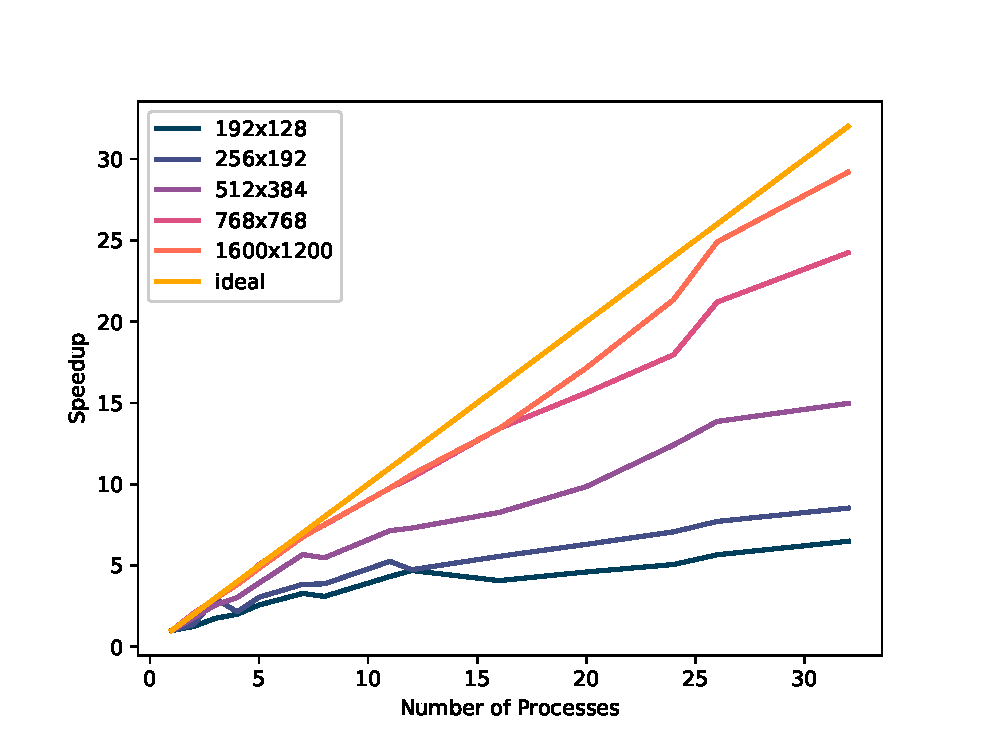
\includegraphics[scale=0.6]{../graphs/Speedup.eps}
                \caption{Speedup for all the input images}
                \label{speedup}
            \end{figure}

            \paragraph{Small Input}
                Ideally as we increase the processors running the speedup should be increased accordingly but this is not the case for small problems. Let's take for example the case where the input image is 192x128 or 256x192 pixels. In Figure 1, it plain to see that the problem doen't scale as it should. When we use even more processors the speedup is slightly inclined. As a result, for the specific size of problems 5 till 12 processes would be the best option. We don't have to waste 10 or 20 more of them if the speedup is not going to exceed 5 and 6 accrodingly.
 
             \paragraph{Medium Input}
                As long as we increase the input image size the speedup is growing faster. From Figure 1 we can denote that for the image 512x384 choosing 26 processes seems a very appealing option. Reaching speedup 13 times faster than running it on one process.

            \paragraph{Big Input}
                In case of input size bigger than 768x768 pixels the results are promising. The speedup is increased almost in a linear fashion, reaching the ideal values and making the communication overhead of the halo swaps to be insignificant. 

        \subsubsection{Average Pixel}
            In this section we have performed analysis for the average pixel results between fixed intervals. Each 100 iterations the average pixel is calculated. In order to achieve that we had to run the experiment till completion for all of the input images. We choose to run them once on for 4 process, because the number of processes has not effect on the average pixel value. This happens due to the fact that the average pixel is depending on the input image and not in how many processes are participation on solving the problem. According to Figure 2, which includes the average pixel values of all input images against the iteration number, it is plain to see that the value is declined in every occassion. That observion is logican due to the fact that the initialized old buffer contain white (255) pixels. As long as the loop is processed the average value is decreasing, meaningly the whole picture is becoming darker. At this point, it worths to mention that in each image from iteration 1 till 100 the pixel value is declined very fast. After that, the change rate is slower, meaning that each iteration has small impact to the new calculated output.

            \begin{figure}[ht]
                \centering
                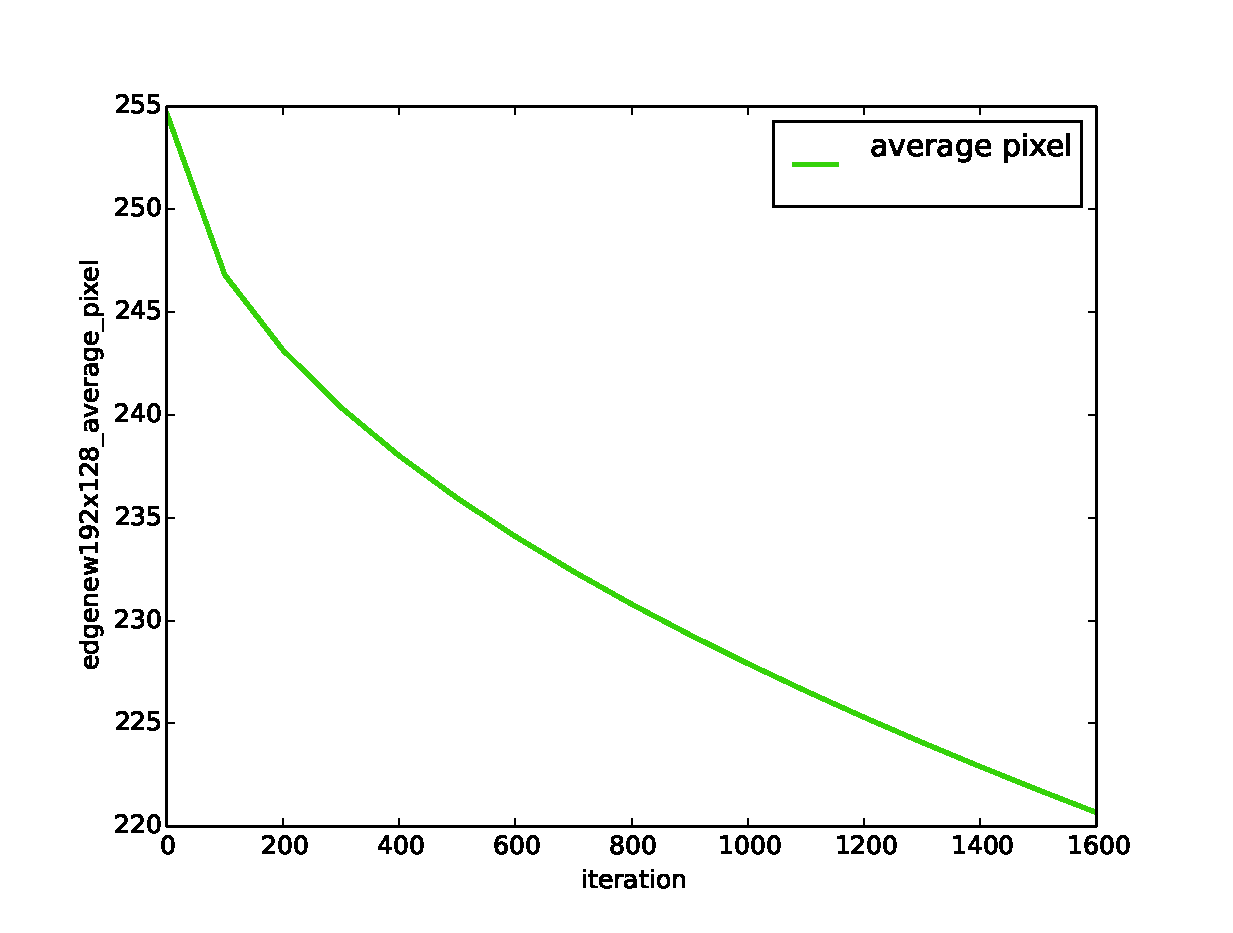
\includegraphics[scale=0.6]{../graphs/edgenew192x128_average_pixel.eps}
                \caption{Average pixel for image 192x128}
                \label{speedup-192x128}
            \end{figure}

\sectionVspacing

\section{Conclusion}
In conclusion.

\end{document}
